\documentclass[11pt]{beamer}

\usetheme{Warsaw}
\usecolortheme{Crane}

\usepackage{amsmath,amssymb}
\usepackage{epstopdf}
\usepackage{graphicx}
\usepackage{enumerate}

\usepackage{bbm}

\newcommand{\ve}{\varepsilon}
\newcommand{\prob}[1]{\mathbb{P}\left[ #1 \right]}
\newcommand{\expect}[1]{\mathbb{E}\!\left[ #1 \right]}
\newcommand{\var}[1]{\mathrm{Var}(#1)}
\newcommand{\cov}[1]{\mathrm{cov}(#1)}
\newcommand{\st}{\text{ s.t. }}

\title{A random graph model of cities}
\author{Joey Huchette and Evan Fields}
\institute{6.268}
\date{May 12, 2015}

\beamertemplatenavigationsymbolsempty
\setbeamercovered{transparent}

\begin{document}

\begin{frame}
\titlepage
\end{frame}

\begin{frame}
\frametitle{Motivation}
Empirical evidence suggests city structure and road coverage powerfully affect population distributions and demand for vehicle miles traveled. We want to see if simple random graph models can capture some of these relationships.
\end{frame}

\begin{frame}
\frametitle{Approach overview}
\begin{enumerate}
\item Create random graph: we represent a city as a finite two-dimensional lattice with random additional edges. The origin represents downtown.
\item Randomly populate the graph: one-by-one residents arrive at the network and decide which node to live at randomly, combining location and density preferences.
\item Compute optimal population: we solve the MIQP of locating residents on the graph to minimize density and travel times under a simple static model.
\end{enumerate}
\end{frame}

\begin{frame}
\frametitle{Random graph creation}
\begin{center}
\includegraphics<1>[width=.5\textwidth]{images/lattice_no_jumps.pdf}
\includegraphics<2>[width=.5\textwidth]{images/lattice_only_jumps.pdf}
\includegraphics<3>[width=.5\textwidth]{images/lattice_with_jumps.pdf}
\end{center}
\begin{enumerate}
\item<1,3> Create a lattice on $[-N,N] \times [-N, N]$
\item<2-> Add $\lfloor N^\alpha \rfloor$ extra edges with one endpoint $u$ chosen uniformly at random and other endpoint $v$ chosen with probability proportional to $d(u,v)^{-\beta}$
\end{enumerate}
\end{frame}

\begin{frame}
\frametitle{Random graph population}
\begin{itemize}
\item $d(v)$: lattice distance from vertex $v$ to the origin
\item $p(v,t)$: population of vertex $v$ at time $t$; $p(\cdot, 1) = 0$
\item $\gamma > 0, \delta > 0$ parameters
\end{itemize}
At times $t = 1, \ldots, M$ a resident arrives at the network and chooses a non-origin vertex to live at with probability proportional to
\[
\frac{1}{d(v)^\gamma \cdot p(v,t)^\delta};
\]
that is, users are likely to select vertices which are close to the origin and have low population.
\end{frame}

\begin{frame}
\frametitle{Optimal population distribution}

Can solve a MIQP to optimally place population on network to avoid overcrowding and traffic congestion.

Take $P(k)$ as the set of all edges through node $k$.

\begin{align*}
	\min\quad& \sum_{k} \left(ax_k + bx_k^2\right) + \sum_{i,j=-N}^N \left(c v_{i,j} + d v_{i,j}^2\right) \\
	\text{s.t.}\quad& x_k = \sum_{(i,j) \in P(k)} v_{i,j} \quad \forall k \\
	& \sum_{i,j = -N}^N v_{i,j} = M \\
	& v_{0,0} = 0 \\
	& v_{i,j} \in \mathbb{Z}_+ \quad \forall -N \leq i,j \leq N
\end{align*}

\end{frame}

\begin{frame}
\frametitle{Average density}
\begin{center}
\only<1>{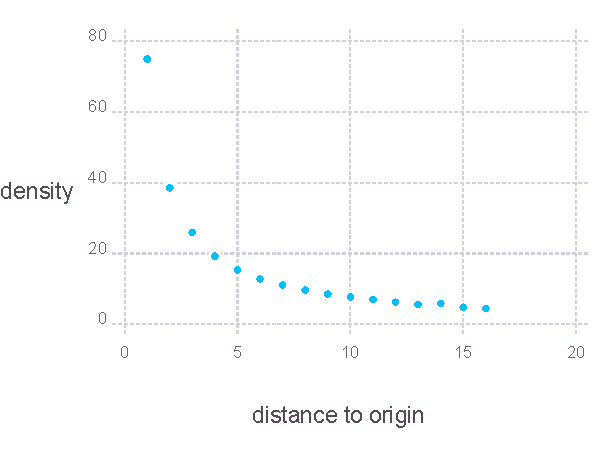
\includegraphics[width=.8\textwidth]{images/density0.pdf}}%
\only<2>{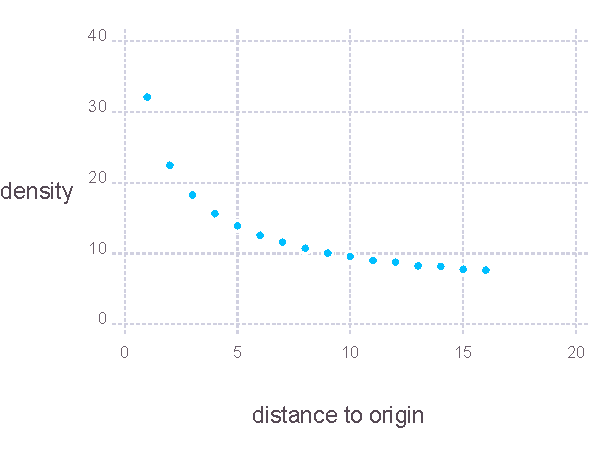
\includegraphics[width=.8\textwidth]{images/density1.pdf}}%
\only<3>{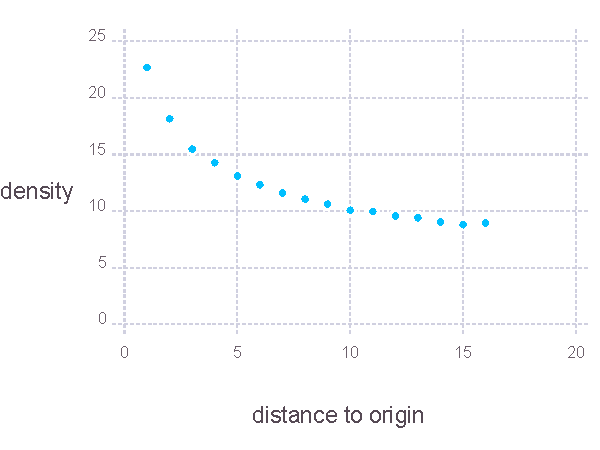
\includegraphics[width=.8\textwidth]{images/density2.pdf}}%
\only<4>{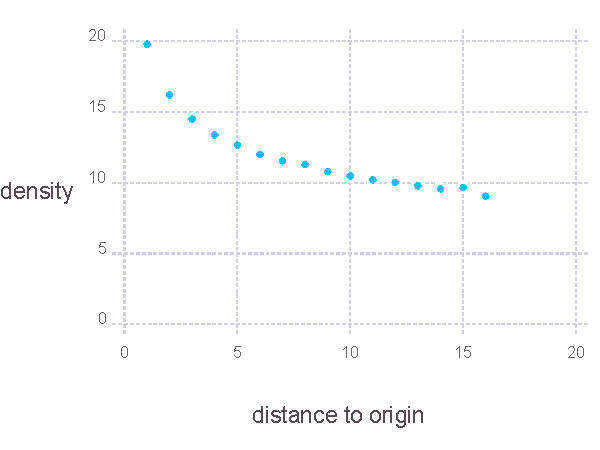
\includegraphics[width=.8\textwidth]{images/density3.pdf}}%

\vspace*{-.2cm}

\only<1>{$\delta = 0$}%
\only<2>{$\delta = 1$}%
\only<3>{$\delta = 2$}%
\only<4>{$\delta = 3$}%

\vspace*{.2cm}

Averaged over 10 replications for a network with $N = 10, \; M = 5000, \; \alpha = 1.5, \; \beta = 1, \; \gamma = 1, \; \delta \in \{0,1,2,3\}$
\end{center}
\end{frame}

\begin{frame}
\frametitle{Example results}
\centering
\only<1>{Average 1 person per vertex}%
\only<2>{Average 10 people per vertex}%
\only<3>{Average 100 people per vertex}%

\includegraphics<1->[width=.3\textwidth]{../plots/distance-1_0-1_5-1-1.pdf}
\includegraphics<1>[width=.3\textwidth]{../plots/individual-1_0-1_5-1-1.pdf}
\includegraphics<2>[width=.3\textwidth]{../plots/individual-1_0-1_5-10-1.pdf}
\includegraphics<3>[width=.3\textwidth]{../plots/individual-1_0-1_5-100-1.pdf}
\includegraphics<1>[width=.3\textwidth]{../plots/optimal-1_0-1_5-1-1.pdf}
\includegraphics<2>[width=.3\textwidth]{../plots/optimal-1_0-1_5-10-1.pdf}
\includegraphics<3>[width=.3\textwidth]{../plots/optimal-1_0-1_5-100-1.pdf}

Distance to origin \hspace*{.6cm} Random location \hspace*{.6cm} Optimal location

\vspace*{.5cm}

For a network with $N = 15, \; \alpha = 1, \; \beta = 1.5, \gamma = \delta = 2$, $a = 0$, $b = 1$, $c = 0$, and $d = 5$.
\end{frame}

\begin{frame}
\frametitle{Example results}
\centering
\only<1>{Average 1 person per vertex}%
\only<2>{Average 10 people per vertex}%
\only<3>{Average 100 people per vertex}%

\includegraphics<1->[width=.3\textwidth]{../plots/distance-2_0-1_5-1-1.pdf}
\includegraphics<1>[width=.3\textwidth]{../plots/individual-2_0-1_5-1-1.pdf}
\includegraphics<2>[width=.3\textwidth]{../plots/individual-2_0-1_5-10-1.pdf}
\includegraphics<3>[width=.3\textwidth]{../plots/individual-2_0-1_5-100-1.pdf}
\includegraphics<1>[width=.3\textwidth]{../plots/optimal-2_0-1_5-1-1.pdf}
\includegraphics<2>[width=.3\textwidth]{../plots/optimal-2_0-1_5-10-1.pdf}
\includegraphics<3>[width=.3\textwidth]{../plots/optimal-2_0-1_5-100-1.pdf}

Distance to origin \hspace*{.6cm} Random location \hspace*{.6cm} Optimal location

\vspace*{.5cm}

For a network with $N = 15, \; \alpha = 2, \; \beta = 1.5, \gamma = \delta = 2$, $a = 0$, $b = 1$, $c = 0$, and $d = 5$.
\end{frame}

\begin{frame}
\frametitle{Conclusion}
\begin{itemize}
	\item Model displays desired decay as distance from origin increases
	\item Myopic preferential attachment displays early transient behavior...
	\item ...that settles to expected distribution
	\item Empirically, appears that larger populations quickly converge to total travel time value strictly greater than minimum possible
\end{itemize}

\end{frame}
\end{document}

